\section{Análisis de diferentes soluciones propuestas}

Vamos a proponer dos escenarios posibles para poder analizar sus soluciones:

\begin{itemize}
    \item Primer escenario:
    $$
    n = 3,\quad
    E=
    \begin{array}{|c|c|c|}
        \hline 
        10 & 2 & 2\\
        \hline 
    \end{array}
    \qquad
    S=
    \begin{array}{|c|c|c|}
        \hline 
        1 & 5 & 4\\
        \hline 
    \end{array}
    $$

    \item Segundo escenario:
    $$
    n = 4,\quad
    E=
    \begin{array}{|c|c|c|c|}
        \hline 
        4 & 3 & 8 & 10\\
        \hline 
    \end{array}
    \qquad
    S=
    \begin{array}{|c|c|c|c|}
        \hline 
        10 & 10 & 10 & 1\\
        \hline 
    \end{array}
    $$
\end{itemize}

Notación: $j$ es la cantidad de días consecutivos de entrenamiento.
De esta manera $s_j$ representa la energía disponible para ese día consecutivo.

Primero procederemos a analizar el primer caso ya que es el proporcionado por la cátedra. En este,
notamos que la ganancia de un día $i$ puede tomar 2 valores posibles:

\begin{itemize}
    \item Suma entre la ganancia del día anterior y el $\min{(e_i, s_j)}$
    \item Suma entre la ganancia de dos días anteriores y el $\min{(e_i, s_1)}$. Esta opción se basa 
    en la suposición de que se realizó un descanso en el día $i-1$.
\end{itemize}

Esto se debe a que hemos observado una relación con el problema de Juan el Vago. En este problema, se cuenta
con un arreglo de ganancias diarias, y Juan busca maximizar su ganancia sin trabajar dos días seguidos. Para
lograr esto, se itera sobre el arreglo observando los días actuales y los dos días anteriores para calcular
la ganancia máxima acumulada.
Si Juan elige trabajar el día $i$, su ganancia sería la suma entre la ganancia del día actual ($g_i$) y
la ganancia de dos días atrás ($g_{i-2}$). En caso contrario, si decide no trabajar, su ganancia sería igual
a la ganancia del día anterior ($g_{i-1}$). De estas dos opciones, se elige la que maximiza la ganancia para
el día $i$.

Esta estrategia nos recuerda al enfoque que estamos explorando en este algoritmo, donde se busca maximizar
la ganancia acumulada eligiendo si conviene o no descansar en el día actual, considerando la energía disponible
y el esfuerzo requerido en cada día.

Relacionando el problema de Scaloni con el problema de Juan el Vago, supusimos erroneamente que para obtener la
ganancia máxima hasta el día $k, \forall k \in [2,n]$ bastaría con calcular la ganancia máxima de los dos días anteriores.
La función de recursión propuesta fue la siguiente:  

$$g(i, j) = \max{\left\{g(n-1) + \min{(e_i,s_j)}, g(n-2) + \min{(e_i,s_1)}\right\}}$$

En relación al caso de tres días que estábamos analizando para ese entonces, cabe destacar que este algoritmo proporcionaba la respuesta esperada, 
que en este contexto era igual a siete.

El inconveniente de este algortimo es que al querer maximizar cada día solo comparando si el día anterior hubiera convenido
descansar o no, no se tiene en consideración el hecho de que hay escenarios donde el descanso es conveniente en un día
$k < i-1$ y solo se hace evidente recién en el día $i$. 

Dado que la ganancia está condicionada por los niveles de energía de cada día consecutivo, en ocasiones es más 
conveniente que la ganancia relativa de un día no sea óptima individualmente, sino que en conjunto 
ofrezca la mayor ganancia posible. El algoritmo propuesto inicialmente no aborda adecuadamente esta complejidad, 
ya que solo considera esta condición con respecto a los dos días anteriores, lo que limita la 
capacidad de adaptación a situaciones donde la estrategia de descanso óptima se extiende en un 
período más largo.

Esto se puede observar en el segundo escenario propuesto. 
Recordamos el escenario 2:
\begin{itemize}
    \item Segundo escenario:
    $$
    n = 4,\quad
    E=
    \begin{array}{|c|c|c|c|}
        \hline 
        4 & 3 & 8 & 10\\
        \hline 
    \end{array}
    \qquad
    S=
    \begin{array}{|c|c|c|c|}
        \hline 
        10 & 10 & 10 & 1\\
        \hline 
    \end{array}
    $$
\end{itemize}


El algoritmo incial 
procede a solucionarlo de la siguiente manera:

$$
\begin{array}{|c|c|c|c|c|c|}
    \hline
    i & \text{j} & \text{ganancia trabajando día i-1} & \text{ganancia sin trabajar día i-1} & \text{ganancia día i} \\
    \hline
    1 & 1 & 4 & 4 & 4 \\
    \hline
    2 & 2 & 4+3 & 0+3 & 7 \\
    \hline
    3 & 3 & 7+8 & 4+8 & 15 \\
    \hline
    4 & 1 & 15+1 & 7+10 & 17 \\
    \hline
\end{array}
$$


Por lo tanto, el resultado obtenido es $17$ descansando en el día $3$, mientras que el resultado
óptimo es $22$, descansando en el día $2$. Este es un claro contraejemplo que ilustra que la decisión
óptima de descansar en el día $2$ no es tomada en consideración ya que no puede deducirse manteniendo
registro de únicamente las ganancias de los dos días anteriores. 

Al darnos cuenta de este problema, procedimos a utilizar una planilla de cálculo para ayudarnos a resolverlo.
Arreglamos $E$ verticalmente y $S$ horizontalmente en un cuadro de doble entrada. Luego, cada
casilla de fila $i$ y columna $j$ es la ganancia parcial que podríamos obtener si ese fuera el $j$-ésimo día
de entrenamiento consecutivo para el día $i$ del plan de entrenamiento. Notamos que la ganancia
máxima hasta el entrenamiento $i$ era el máximo de las ganancias parciales de la misma fila.
Decidimos entonces colocar a la izquierda una columna auxiliar que contenía la ganancia maxima
de la fila inferior. Ver resultado en la figura \ref{fig:planilla_caso_2}.

\begin{figure}[H]
    \centering
    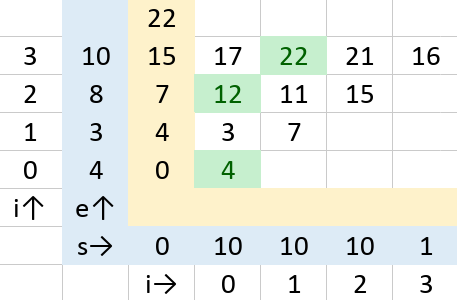
\includegraphics[width=0.5\textwidth]{img/planilla_caso_2.png}
    \caption{Caso 2 planilla}
    \label{fig:planilla_caso_2}
\end{figure}

Luego, logramos abstraer las funciones, mostradas en la figuras \ref{fig:formulas_planilla_1},
\ref{fig:formulas_planilla_2} y \ref{fig:planilla_completa}.

\begin{figure}[ht]
    \centering
    \begin{minipage}[b]{0.495\textwidth}
        \centering
        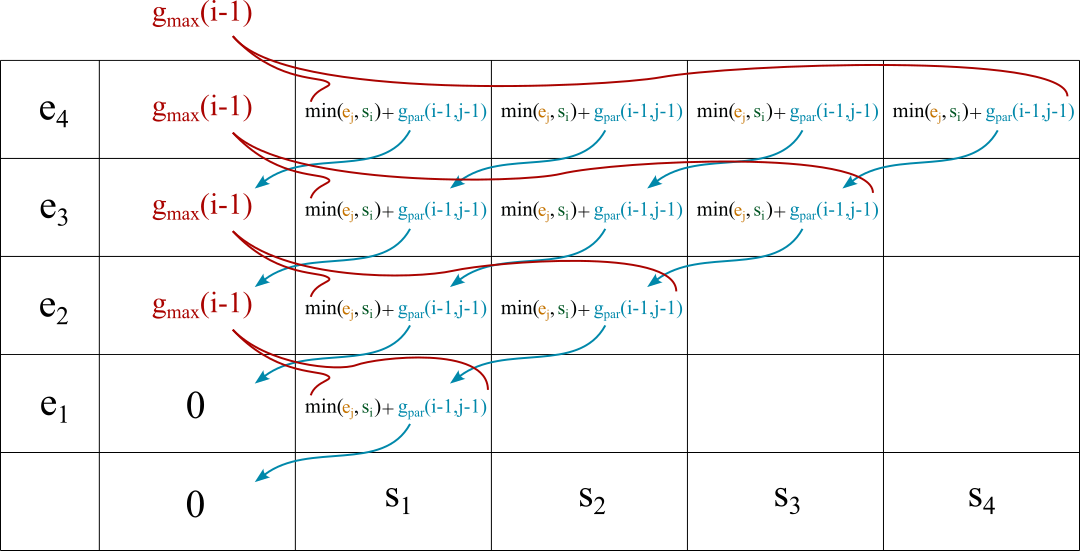
\includegraphics[width=\textwidth]{img/formulas_planilla_1.png}
        \caption{Formulas en planilla a}
        \label{fig:formulas_planilla_1}
    \end{minipage}
    \begin{minipage}[b]{0.495\textwidth}
        \centering
        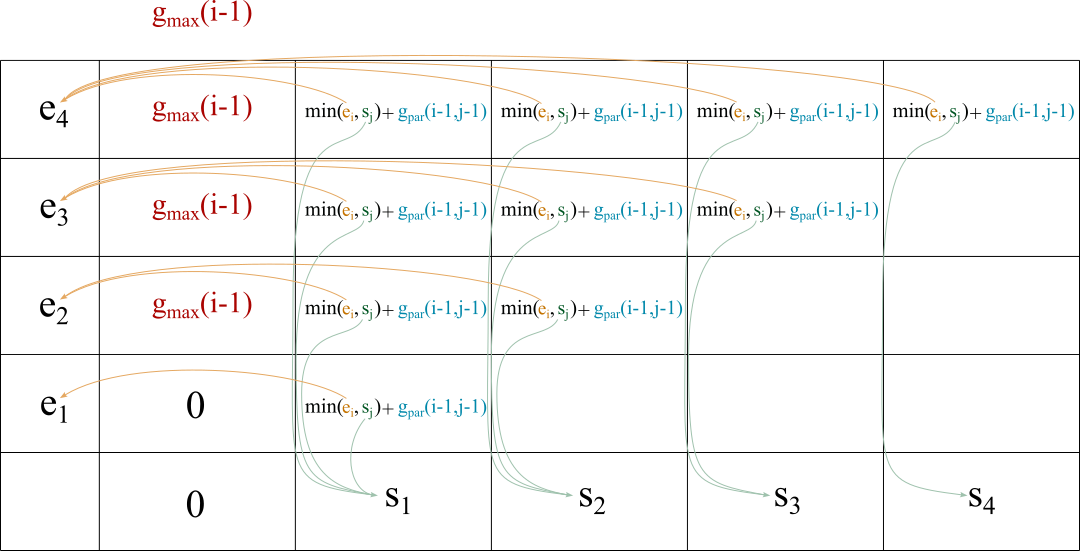
\includegraphics[width=\textwidth]{img/formulas_planilla_2.png}
        \caption{Formulas en planilla b}
        \label{fig:formulas_planilla_2}
    \end{minipage}
\end{figure}

\begin{figure}[H]
    \centering
    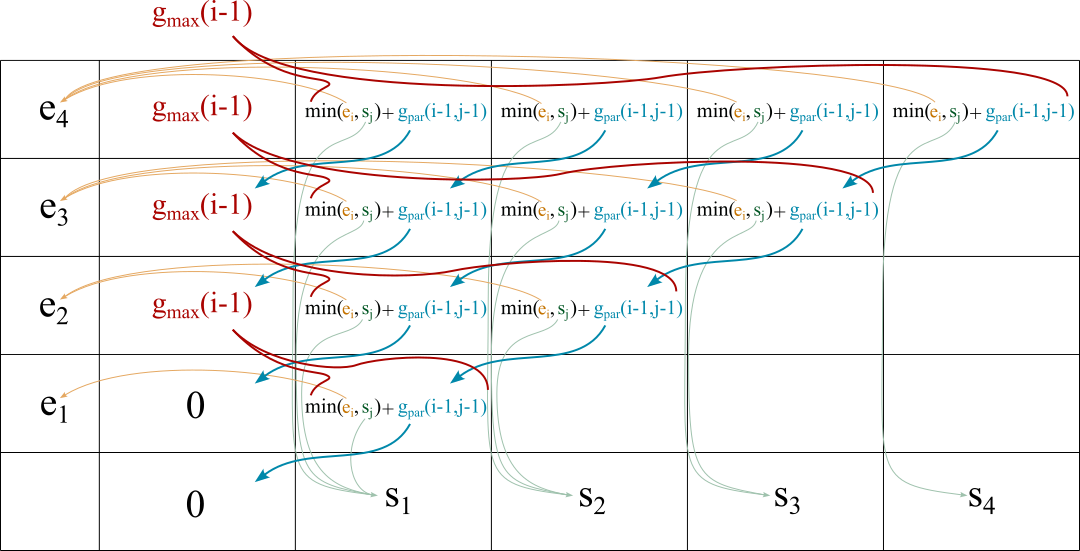
\includegraphics[width=1\textwidth]{img/planilla_completa.png}
    \caption{Formulas en planilla}
    \label{fig:planilla_completa}
\end{figure}

Basándonos en esta planilla, pudimos abstraer la solución.

\section{Solución final}

A continuación procederemos a describir el algoritmo que soluciona la problemática de Scaloni de
manera óptima desarrollado con la ténica de diseño: Programación Dinámica.

\subsection{Función de recurrencia}

Sea $s_{j}$ la energía restante para $j$ días consecutivos de entrenamiento y
$e_{i}$ la cantidad de esfuerzo del entrenamiento $i$.

El problema nos da dos arreglos de tamaño $n$:

$$
S = (s_{1},s_{2},\dots ,s_{n}) \quad E=(e_{1},e_{2},\dots ,e_{n})
$$

Definimos la función $g(i,j)$ como la ganancia obtenida del $i$-ésimo entrenamiento,
dado que estamos en el día $j$ de entrenamiento consecutivo.

$$
g(i,j)=\min{(e_{i},s_{j})}
$$

Definimos la función $g_{par}(i,j)$ como la ganancia parcial acumulada hasta el $i$-ésimo entrenamiento
dado que estamos en el día $j$ de entrenamiento consecutivo.
$$
\forall j\leq i,\  g_{par}(i,j)=\begin{cases}
0 & i=0 \\
g(i,j) & i=1 \\
g(i,j)+g_{max}(i-2) & i>1 \land j=1 \\
g(i,j)+g_{par}(i-1,j-1) & i>1 \land j>1
\end{cases}
$$

Finalmente, definimos la función $g_{max}(i)$ como la ganancia máxima obtenida hasta el $i$-ésimo
entrenamiento, que es la solución al problema de la consigna.

$$
g_{max}(i)=\max{\left\{ g_{par}(i,j) \right\}_{j\leq i}}
$$

\subsection{Solución iterativa}

Como podemos observar en la sección anterior, la solución es recursiva. Implementarla de esta forma sin
optimizaciones requeriría mucho recálculo. Esto puede ser solucionado con memoization y la implemantación más
simple es de forma iterativa y bottom-up.

Definimos la función \texttt{optimizar\_entrenamiento} que recibe como parámetro \texttt{n}, un arreglo con los esfuerzos requeridos
en los entrenamientos y otro con las energías disponibles por días de entrenamiento consecutivo. Devuelve la ganancia máxima y un array
con el plan de entrenamiento óptimo.

\begin{lstlisting}[language=Python]
def optimizar_entrenamiento(n, esfuerzos, energias):
    ganancias_parciales = _ganancias_parciales(n, esfuerzos, energias)
    ganancia_maxima = _ganancia_maxima(ganancias_parciales)
    plan_entrenamiento_optimo = _plan_entrenamiento_optimo_2(ganancias_parciales)
    return ganancia_maxima, plan_entrenamiento_optimo
\end{lstlisting}

La función \texttt{\_ganancias\_parciales(n, esfuerzos, energias)} genera una lista de longitud $n$ donde
la casilla $i$ es una lista de longitud $i$ con las ganancias parciales de cada día de entrenamiento
consecutivo $j$. Se construye bottom-up, es decir, primero se calculan las ganancias
parciales para el entrenamiento $1$, luego para el $2$ y así sucesivamente hasta el $n$.

Luego, \texttt{\_ganancia\_maxima(ganancias\_parciales)} devuelve el máximo de las ganancias parciales de la
última fila.

Finalmente, \texttt{\_plan\_entrenamiento\_optimo(ganancias\_parciales)} reconstruye el plan de entrenamiento
óptimo a partir de la lista de ganancias parciales. Para esto, recorre la lista de ganancias parciales desde
el final al principio. Parte de la ganancia parcial máxima de la última fila y baja en diagonal hasta la
primera columna. Esta se refiere a entrenar ese día siendo el primer día de entrenamiento consecutivo, lo que
implica que el día anterior se descanzó. Por esto, se salta la fila siguiente, continuando normalmente, 
partiendo de nuevo desde la ganancia parcial máxima y bajando en diagonal. Repite estos pasos hasta
llegar a la primera fila.
